\chapter{System Description}
\label{systemdescription}
\paragraph{}
Following the study of the above works related to Word Sense Disambiguation, we find the need to build a system, which is directed at minimizing the size of the training model and the time taken to predict word senses, more significant. For that, we populated the following characteristics that we want in our system:
\begin{enumerate}
\item Requires minimal pre-processing for training and test inputs
\item Training model must be small, and easy to interpret
\item Perform speedily
%%from Aobo:\item Reasonable accuracy. a fast and small system also doesn't make sense when the performance is poor.
\end{enumerate}

\paragraph{}
Decision Trees is one of the simplest predictive model and thus it is simple to interpret and understand. It requires little data preparations, and able to have value even with little hard data. It is able to process large amount of data in a short time. With that, we decided to implement our system using Decision Trees. We use the Weka\footnote{http://www.cs.waikato.ac.nz/ml/weka/} implementation of the J48 decision tree learner to generate the model files to help us predict word senses.
%%From Chen Tao:Here you mention the system use J48, but in chapter2.5 and in chapter3.4, you use C4.5. You may explain that J48 is an open source Java implementation of the C4.5 algorithm in the weka data mining tool. Otherwise, people may think that they are two different decision trees. Another suggestion is "It requires little data preparations, and able to have value" may need to revise into "It requires... and is able to..."

\paragraph{}
The intuition of our method is that a sentence is the \textit{environment} that helps determine the word senses of ambiguous words. Consider a simple case where there is only one target word that needs to be disambiguated. We look at the surrounding words in the same sentence, such that if there exists a particular set of determining words, we predict that the target word would possess a specific word sense.

\paragraph{}
We used the \textsc{SemCor1.7.1} corpus as our training data set. We used the tagged Brown Corpus files that have all content words tagged. We were able to identify a total of 20450 \textit{lemmas}. By \textit{lemma} we refer to the root form of a word.  For example, the root form for the word ``ate'' is ``eat'', and root form for ``runs'' is ``run''. We predict word senses based on the sense keys extracted for these lemmas. Since our approach predicts word senses by looking at the entire sentence, we parsed the training corpus and saved it into numerous sentences. Then for each lemma, we save a sentence as an \textit{instance} for that lemma if the sentence contains that lemma.

\paragraph{}
For each lemma, we generated the model files with pruning to remove any irrelevant branches in the trees. Moreover, it%%Aobo: what does it refer to?
 reduces the size of the trees, and will be even smaller and more efficient to store and use. In these model files there are \textbf{2261} trees that are \textit{unary}, that it is simply a leaf node, and  captures only one result for word sense. After checking against the original corpus, it was found that these unary files were simply due to the fact that these lemmas had only one instance of occurrence in the corpus and thus only one word sense. For the other trees, their \textit{depths} range from \textbf{5 to 49}, and the number of \textit{leaf nodes} ranges from \textbf{2 to 25}. Figure \ref{fig:treeAdvance} shows an example of the tree structure (definitions in brackets are displayed only for illustration purpose).

\begin{figure}[h]
  \centering
  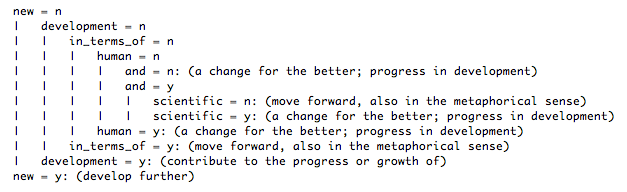
\includegraphics[scale=0.75]{./advance}
  \caption{Tree for \textit{advance}}
  \label{fig:treeAdvance}
\end{figure}

%\subsection{Training Data Set}
%\label{trainingdataset}
%\paragraph{}
%We make use of the widely used \textsc{SemCor}[to be cited] for our training data set. Specifically we use the tagged Brown Corpus files, with all content words tagged, of \textsc{SemCor}1.7.1. From this training data set, we retrieved a total of 20450 lemmas. Each lemma has a collection of sentences that that contain the lemma itself. Each sentence is an instance of the \textit{environment} that determines the word sense of that lemma. To capture these information, each lemma has an ARFF file, with all the words in the sentences as the \textit{attributes}, and the sentences themselves as the \textit{data instances}. In addition, we added an additional attribute to each ARFF file, \textit{WordNetSenseKey}, which captures the corresponding word sense for each data instance.

%\paragraph{}
%To generate the ARFF files for a target word, we first extract all sentences that contain the target word. We retain the WordNet sense key information found in the \textsc{SemCor} tagged files, and also the words' occurrence form. What follows is to specify each non-target word as an \textit{attribute} of its ARFF file, and each \textit{data instance} would represent each sentence. Each of these attributes would only have a true or false value, representing whether it exists in a particular sentence. Last, we add an additional attribute, \textit{WordNetSenseKey}, which captures the list of all sense keys available for that target word in the tagged files. \\
%\begin{figure}[htbp]
%@relation act \\ \\
%@attribute It \{\textit{n,y}\} \\
%@attribute recommended \{\textit{n,y}\} \\
%$\vdots$ \\
%@attribute WordNetSenseKey \{\textit{key 1},\textit{key 2}, $\ldots$ , \textit{key n}\} \\ \\
%@data \\
%\textit{y,y,n, $\ldots$ ,key 5} \\
%$\vdots$
%\caption{Sample ARFF file, \textit{act.arff}}
%\label{fig:sampleArff}
%\end{figure}
%\begin{figure}[htbp]
%  \centering
%  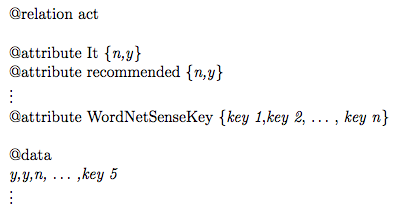
\includegraphics[scale=0.7]{./arff}
%  \caption{Sample ARFF file, \textit{act.arff}}
%  \label{arff}
%\end{figure}

%\paragraph{}
%On the side note, we saved the actual WordNet sense key in a separate location in order to keep the ARFF file free from attribute values that contains too many characters. For example, for \textit{act.arff}, the last attribute would only have values $1,2,\ldots,n$. The actual sense keys are saved in \textit{act.senselist}, which has a corresponding list of sense keys.

\section{Predicting Word Sense}
%\paragraph{}
%To predict the word sense of a target word, our system makes use of the sentence, which a target word occurred in, as the ``environment'', in other words context, of the word itself. The existence of certain words would contribute to an ambiguous word's sense in that sentence itself. For instance, consider the word \textit{bank}. It is logical, that if a sentence with the word \textit{bank} also contains the word \textit{interest} or \textit{financial}, we know that \textit{bank} here is \textit{likely} to refer to the place where we would have a savings account etc. In other case where the sentence contains \textit{river}, we can probably go fishing at this \textit{bank}.
\paragraph{}
Prediction of a target word begins with capturing the entire sentence the target word resides in. This is the \textit{environment} we mentioned in our intuition. 
Consider a sentence with only one ambiguous word to be disambiguated.%% Aobo: no connection between these two sentences 
 So we use the rest of the sentence to predict the word sense of that target word. Consider a set of all English words, $\varepsilon = \{$all English words\}. Ignoring the order of words and repeated usage of the same word in the same sentence, an English sentence can be denoted as a set of English words, as such: $S_{i} = \{a_{1}, a_{2}, \ldots, a_{k}\},~S\subseteq \varepsilon$. Therefore, suppose we perform WSD on $a_{j}$, we consider the set $S - \{a_{j}\}$ as its \textit{environment} that determines its word sense.

%\paragraph{}
%The next step is to create a data instance, and test it against an existing ARFF file. We first lemmatize $T$, then we check whether an ARFF file for the lemma $T_{lemma}$ exists. Suppose it exists. Then we generate a temporary ARFF file for $T_{lemma}$, such that its attributes are the same as the existing one in the training data set. Finally we use this temporary ARFF file to test against the training file, and hence outputs the prediction from our system.

\paragraph{}
In order to test for $a_{j}$, we check our training data set for existing data about $a_{j}$. Using the set $S_{i} - \{a_{j}\}$, we generate a single data instance to test against our training data. From there we utilize the Weka's Java packages to predict the word sense of $a_{j}$.

\paragraph{}
We test our system for the \textsc{SensEval} and \textsc{SemEval} all-words tasks. We pre-processed the test corpus such that we were able to test sentence by sentence. For all the sentences, we removed all quotations and punctuations, retaining only the English words as we only consider the actual words for word sense predictions.

\paragraph{}
In the following sections, we describe our implementation of the system in iterations. We will also provide the test results at each respective stage. We conducted our experiments using \textsc{SemCor1.7.1} as the training corpus for all the test corpus we were testing against. Our \textit{Baseline} is the WordNet-Sense-One, which assigns the most frequently tagged sense as the answer. The results of the WSD accuracies are shown in Table \ref{tab:resultsSum}.
%%From Chen Tao:  In Table3.3 you use WNs1 as the abbreviation of WordNet-Sense-One, it will be better if you explicitly write the abbreviation here.

\section{Iteration 1 (DT v0.1)}
\label{it:1}
\paragraph{}
Suppose we are performing WSD for every word in a sentence, a single-instance test file is generated for every testable word in the sentence. Then for each test file we run the prediction process to get the word sense. Consider the following example: \\

\begin{figure}[h]
\center
Before: the \textbf{quick} \textbf{brown} fox jumps \textbf{over} the lazy \textbf{dog} \\
\hspace{18 mm}After: the \textbf{quick}(\textbf{1}) \textbf{brown}(\textbf{1}) fox jumps \textbf{over}(\textbf{2}) the lazy \textbf{dog}(\textbf{1})
\caption{Output from iteration DT v0.1}
\end{figure}

\paragraph{}
In this example, the bold words are ambiguous, and we run them through the prediction process. The numbers in brackets are the results of the prediction process, and each of them refers to their corresponding word sense. The actual sense keys are stored in a different location to make the output cleaner.

\paragraph{}
In this iteration, the only feature we used is the occurrence of the neighboring words of a testable word, the \textit{environment} as we defined. As we were experimenting on this iteration, we quickly noticed that the speed of the prediction process was very slow. On average, the time taken to perform WSD on a sentence can easily be \textbf{10 to 40 seconds}. We picked a few random sentences from the test corpus to make comparison with the IMS system by \cite{itmakessense}, and the IMS performs at least 70\% faster than our system. Also, we compared our model size with IMS's, and our system's model size was twice as large (refer to Table \ref{tab:modelSize}). We address this two issues in Iteration 2.

\begin{table}[h]
	\center
	\begin{tabular}{| c | c |}
		\hline
		& Model Size \\
		\hline
		IMS & $\approx$ 275MB \\
		\hline
		DT v0.1 & $\approx$ 545MB \\
		\hline
	\end{tabular}
	\caption{Model size comparison}
	\label{tab:modelSize}
\end{table}

%\paragraph{}
%In this implementation, we make predictions using the model files generated using the J48 classifier. However, when we compared our model files with the model files of the IMS system, we found it to be 2 times as large (refer to Table \ref{tab:modelSize}). We concluded that in our model files, there are too much redundant information that is not used during the prediction process.

%\paragraph{}
%In our training data, information are captured in the form ARFF files. The attributes in these files are all the non-target words of the sentences. We captured these words as they are, and we did not perform lemmatization on them.

\section{Iteration 2 (DT v0.2)}
\label{it:2}
\paragraph{}
We found that in our model files, there are a lot of information that we can omit. More specifically, we only require the actual \textit{tree} itself for the prediction process, like the one illustrated in Figure \ref{fig:treeAdvance}. Hence we extracted only these trees, and further compacted the output such that each tree is now represented in a single line, as illustrated here:
\begin{center}
\textbf{advance$>$}new=n!$|$development=n!$||$in-terms-of=n!$|||$human=n!$||||$and=n:1(4/1)!$||||$and=y!$\ldots$
\end{center}

\paragraph{}
With this we compacted all trees into a single file, having the size of approximately \textbf{1 MB}. At this point, we were able to keep our model size very small, and to fulfill one of our goals: Size of Model.

\paragraph{}
Since the format of the model files was modified, the prediction procedures were also modified. In the modified procedures we dropped the usage of Weka to process the test instance. So we also did not need to generate a temporary test instance file to test against the existing file in our system. Instead, we used the trees extracted and treated each node as a test condition. So prediction means testing against nodes of the tree, eventually leading to a leaf node that provides a word sense.

\paragraph{}
We evaluated this iteration of our system to first make sure that the WSD accuracy remain the same, and also to determine the time taken. In the previous version, the prediction process for just one sentence can easily take 10-40 seconds, depending on length of the sentence. In the new procedure, all the trees are captured within a single file and we load the entire file into memory during the prediction process, in the form of a hash. With that, we were able to process all sentences from the three test corpus we tested against in approximately 2 minutes, averaging at about \textbf{0.10 seconds} per sentence. Compared to the previous iteration, we were able to reduce the time taken by at least \textbf{98\%}. With that we had also fulfilled the other goal: Speed.

\begin{table}[h]
	\center
	\begin{tabular}{| l | c | c |}
		\hline
		& Before DT v0.2 & DT v0.2\\
		\hline
		Model Size (MB) & 545 & \textbf{\large{1}} \\
		\hline
		Time Taken (secs per sentence) & 10 to 40 & \textbf{\large{0.10}} \\
		\hline
	\end{tabular}
	\caption{Comparison of model size and time taken}
	\label{tab:spaceandtime}
\end{table}

\section{Iteration 3 (DT v0.3)}
\label{it:3}
\paragraph{}
In the previous iteration, we did not lemmatize the attributes in our training data files. We speculated that if we lemmatize the attributes, we should be able to get better results compared to the previous implementation. By lemmatizing the attributes, we remove redundant attributes. For example, ``ate'' and ``eat'', where ``ate'' is considered redundant, since our system does not consider the tense of words. By doing so we also remove redundant nodes in the trees generated from the decision tree learner. For that the size of the new model trained from a new version of training data set was further reduced by \textbf{2\%}, from 1,052,703 to 1,032,414 bytes. Zooming in to each lemma's tree, we have reduction of tree sizes of up to \textbf{22\%}.

\begin{table}
	\begin{tabular}[h]{| l | c | c | c |}
		\hline
		& \textsc{SensEval-2} (\%) & \textsc{SensEval-3} (\%) & \textsc{SemEval-2007} Coarse-Grained (\%) \\
		\hline
		%Baseline & 62.4 & 58.9 & 73.0 \\
		Baseline (WNs1) & 55.9 & 48.8 & 64.3 \\
		\hline
		%DT v0.1 & 51.3 & 48.8 & \textbf{78.9} \\
		DT v0.1 & 48.5 & 45.5 & 57.8 \\
		\hline
		%DT v0.2 & 55.1 & 49.4 & 79.3 \\
		DT v0.2 & 48.5 & 45.5 & 57.8 \\
		%\hline
		%DT v0.1 + confidence & 54.8 & 50.1 & 79.3 \\
		\hline
		DT v0.3 & 49.2 & 46.2 & 58.3 \\
		\hline
		IMS & 68.2 & 67.6 & 82.6 \\
		\hline
	\end{tabular}
	\caption{WSD accuracies on \textsc{SensEval} and \textsc{SemEval} all-words tasks}
	\label{tab:resultsSum}
\end{table}

\paragraph{}
In this iteration we also added the \textit{confidence} feature, whereby if the confidence in the prediction is too low%%bellow a threshold 0.5?? give the number 
, we will switch to using the first sense of WordNet, that is, the sense with most frequency count. The value of confidence ranges from 0 to 1. As illustrated in Figure \ref{fig:outputDTv0.2}, the confidence values are now reflected alongside the prediction.

\begin{figure}[h]
\begin{flushleft}
\vspace{5 mm}
\hspace{10 mm}Before: the \textbf{quick} \textbf{brown} fox jumps \textbf{over} the lazy \textbf{dog} \\
\hspace{10 mm}After: the \textbf{quick}(\textbf{1:0.71}) \textbf{brown}(\textbf{1:0.97}) fox jumps \textbf{over}(\textbf{2:0.92}) the lazy \textbf{dog}(\textbf{1:0.98})
\end{flushleft}
\caption{Output from iteration DT v0.2}
\label{fig:outputDTv0.2}
\end{figure}

\paragraph{}
We evaluated our system with this new iteration and we attained improvements for all the corpus we tested against (refer to Table \ref{tab:resultsSum}). With this we demonstrated that even with a reduction of model size, we were able to attain an improvement in WSD accuracy.

\paragraph{}
For the time taken to perform WSD, we evaluated our system against the IMS system. Our system's model size is approximately 1MB, whereas IMS's is about 275MB. During the WSD process, both systems would need to load their models into memory. Clearly, loading IMS's model would take a longer time. In order for the comparison to be more fair, the number of test sentences have to be large enough so that the loading time would be less significant in the total amount of time taken. For that we use all the sentences we parsed from the test corpus, \textsc{SensEval-2}, \textsc{SensEval-3} and \textsc{SemEval}, to form a single test file of \textbf{789} sentences.

\begin{table}[h]
\center
\begin{tabular}{| c | c | c |}
\hline
& IMS & DT v0.3 \\
%& DT v0.3 Modified \\
\hline
For 789 sentences & 50.322 secs & 81.148 secs \\
%& \textbf{46.074 secs} \\
\hline
Time Taken per sentence & 0.0637 secs & 0.103 secs \\
%& \textbf{0.0584 secs} \\
\hline
\end{tabular}
\caption{Speed Test Experiment 1}
\label{tab:speedTest}
\end{table}

\paragraph{}
Our system loads the model into memory every time it performs WSD on a new sentence. For IMS, its model files are loaded only once to perform WSD on all 789 sentences. The time taken for this speed test is summarized into Table \ref{tab:speedTest}. Clearly, when performing WSD on large amount of text, IMS performs about \textbf{38\%} faster when compared with DT v0.3.
\paragraph{}
However this is not the intended nature for our system. Our system is meant to only perform WSD on a single sentence. In order to illustrate how our system actually performs, we need to perform a second speed test.

\begin{table}[h]
\center
\begin{tabular}{| c | c | c |}
\hline
& IMS & DT v0.3 \\
\hline
For 62 sentences & 17.636 secs & \textbf{\large{7.611 secs}} \\
\hline
Time Taken per sentence & 0.284 secs & \textbf{\large{0.123 secs}} \\
\hline
\end{tabular}
\caption{Speed Test Experiment 2}
\label{tab:speedTest2}
\end{table}

\paragraph{}
In this second speed test, we picked \textbf{62} random sentences from the test corpus. We ran these sentences through both system for \textbf{10} rounds each, and computed the average score for each round. For this speed test, we used the original DT v0.3 to compare against IMS. Making reference to the figures in bold in Table \ref{tab:speedTest2}, our system is faster in this speed test, when the setting is only to test for small amount of text. The speed performance of our system fulfills one of our goals: Speed. 